\documentclass[11pt]{article}
\usepackage[margin=1in]{geometry}
\usepackage{booktabs}
\usepackage{graphicx}
\usepackage{subcaption}
\usepackage{minted}
\usepackage{xcolor}
\usepackage{float}
\usepackage[hidelinks]{hyperref}

\setminted{fontsize=\footnotesize, breaklines, frame=single,
framesep=2mm, linenos}
% \codefile{<lexer>}{<title>}{<path>}
\newcommand{\codefile}[3]{\par\noindent\texttt{\small #2}\inputminted{#1}{#3}}

\newcommand{\nVertices}{76,269}
\newcommand{\nEdges}{1,762,504}
\newcommand{\nComponents}{1}

\setlength{\tabcolsep}{4pt}

\title{CS 6350 Assignment 3\\\large Spark Structured Streaming with
Kafka/ELK \& GraphFrames}
\author{Nico OR}
\date{\today}

\begin{document}
\maketitle

%======================================================================
\section{Part 1: Named-entity counts from a real-time news stream}

\subsection{Data source}
The real-time source is \textbf{NewsAPI} (\url{https://newsapi.org}), queried
through the \texttt{newsapi-python} client. A poller service calls the
top-headlines endpoint with parameters language=en, country=us,
category=business, that is,  Business news in english from American
publications, news every 900 seconds, or every 15 minutes. For each
article, the title, description and HTML-stripped content snippet are
concatenated and written to the Kafka topic articles. Headlines
already sent in this run are stored in a python set and not posted to
the Kafka topic after their first appearence, so repeated polls do
not double count the same story.

\subsection{Pipeline}
\begin{enumerate}
  \item \textbf{Poller} (Python, \texttt{kafka-python}) $\rightarrow$
    Kafka topic \texttt{articles}.
  \item \textbf{Processor} (PySpark Structured Streaming) reads
    \texttt{articles},
    extracts named entities with a spaCy (\texttt{en\_core\_web\_sm}) UDF,
    explodes them, and keeps a running \texttt{groupBy(entity).count()}.
    Every 30\,s trigger (in \texttt{complete} output mode) the full table of
    \texttt{\{"entities", "count"\}} JSON records is written to the Kafka topic
    \texttt{logs.entities} (topic2).
  \item \textbf{Logstash} subscribes to every \texttt{logs.*} topic
    and indexes the
    records into Elasticsearch index \texttt{logs.entities-YYYY.MM.dd}.
  \item \textbf{Kibana} bar chart: X-axis = top 10 terms of
    \texttt{entities.keyword}, ordered by Y-axis = \emph{max} of \texttt{count}.
    Each trigger appends a new document with the cumulative count, so the
    maximum count per entity in the time window is the running count at the
    end of the window.
\end{enumerate}
All components (Kafka 4.4.0 in KRaft mode, Elasticsearch/Logstash/Kibana 9.5.5,
the poller and the processor) run as containers from
\texttt{kafka-elk/compose.yaml}.

\subsection{Results}
The stack was started from empty volumes at 18:44:16 CST on 2026-11-16
($t=0$). The Kibana chart was captured at $t = 15, 30, 45, 60$ minutes, each
60\,s after the mark so the poll landing on that boundary was already indexed.
The time window of each chart runs from start-up to the capture time.
Tables~\ref{tab:ent15}--\ref{tab:ent60} list the same top-10 values, read
directly from Elasticsearch.

\begin{figure}[H]\centering
  \begin{subfigure}{0.49\linewidth}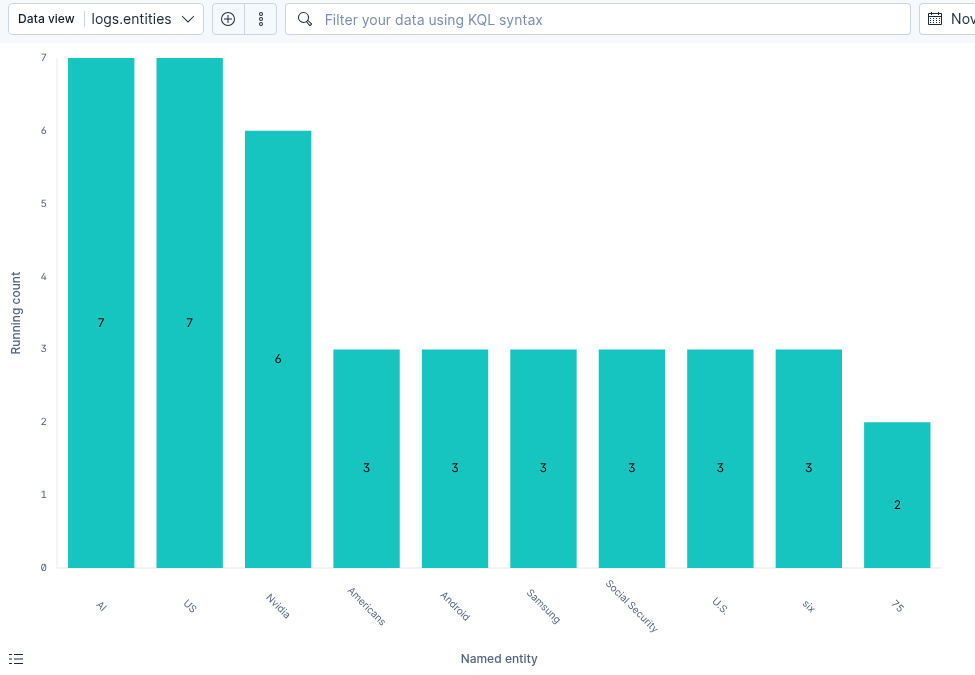
\includegraphics[width=\linewidth]{outputs/kibana_top10_15min.png}\caption{$t=15$
    min}
  \end{subfigure}\hfill
  \begin{subfigure}{0.49\linewidth}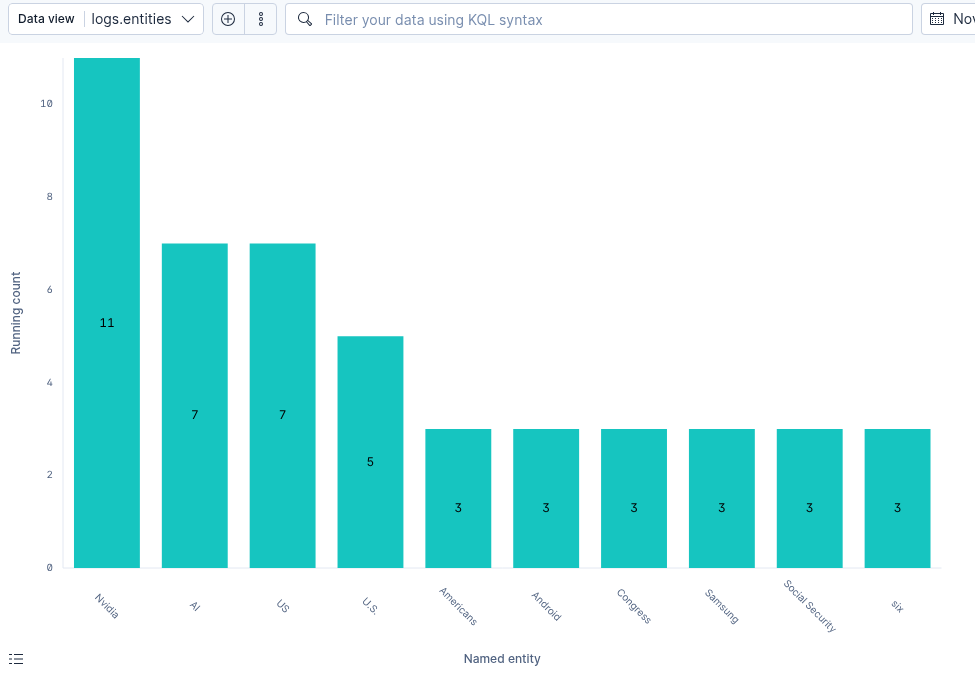
\includegraphics[width=\linewidth]{outputs/kibana_top10_30min.png}\caption{$t=30$
    min}
  \end{subfigure}

  \begin{subfigure}{0.49\linewidth}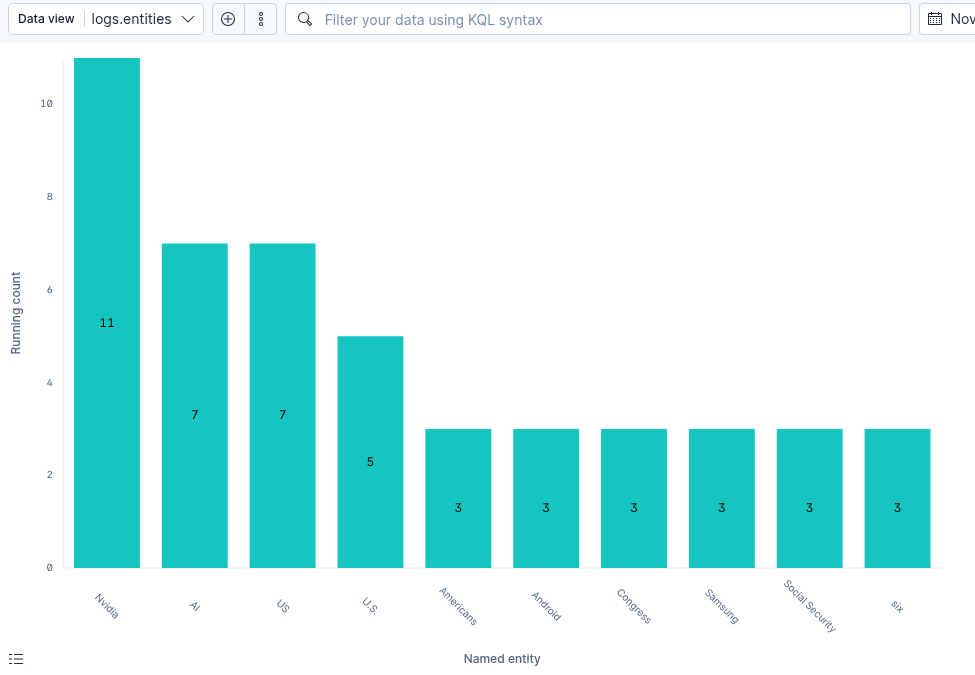
\includegraphics[width=\linewidth]{outputs/kibana_top10_45min.png}\caption{$t=45$
    min}
  \end{subfigure}\hfill
  \begin{subfigure}{0.49\linewidth}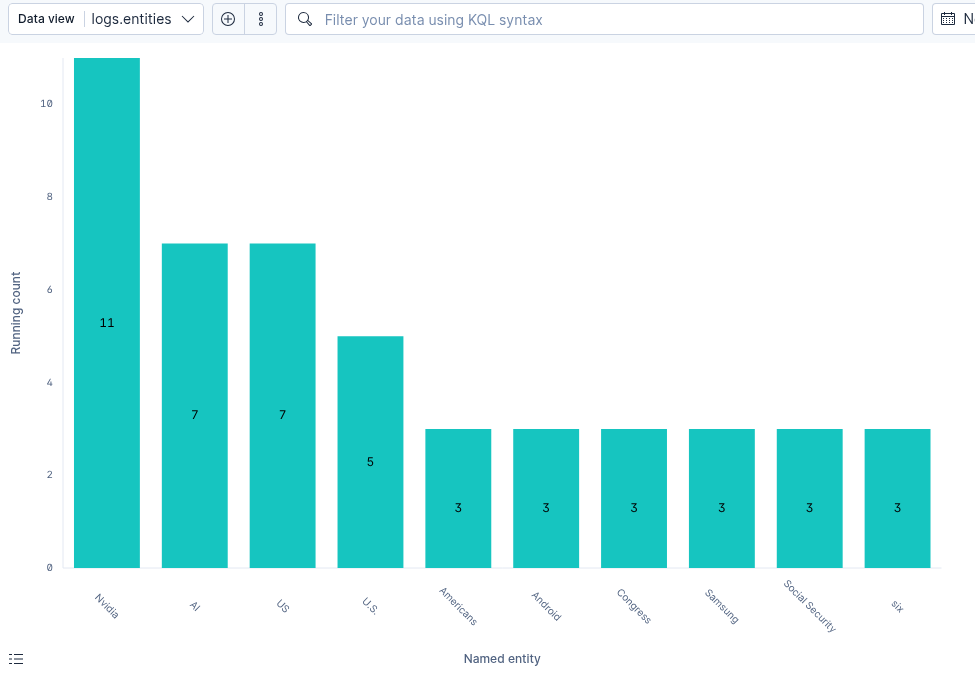
\includegraphics[width=\linewidth]{outputs/kibana_top10_60min.png}\caption{$t=60$
    min}
  \end{subfigure}
  \caption{Kibana bar plots of the top 10 named entities (running
  count) after 15, 30, 45 and 60 minutes.}
  \label{fig:kibana}
\end{figure}

\begin{table}[H]\centering\footnotesize\setlength{\tabcolsep}{3pt}
  \begin{subtable}[t]{0.45\linewidth}\centering\begin{tabular}{rlr}
\toprule
Rank & Entity & Count \\
\midrule
1 & AI & 7 \\
2 & US & 7 \\
3 & Nvidia & 6 \\
4 & Americans & 3 \\
5 & Android & 3 \\
6 & Samsung & 3 \\
7 & Social Security & 3 \\
8 & U.S. & 3 \\
9 & six & 3 \\
10 & 75 & 2 \\
\bottomrule
\end{tabular}
\caption{15
    min}\label{tab:ent15}
  \end{subtable}\hfill
  \begin{subtable}[t]{0.45\linewidth}\centering\begin{tabular}{rlr}
\toprule
Rank & Entity & Count \\
\midrule
1 & Nvidia & 11 \\
2 & AI & 7 \\
3 & US & 7 \\
4 & U.S. & 5 \\
5 & Americans & 3 \\
6 & Android & 3 \\
7 & Congress & 3 \\
8 & Samsung & 3 \\
9 & Social Security & 3 \\
10 & six & 3 \\
\bottomrule
\end{tabular}
\caption{30
    min}\label{tab:ent30}
  \end{subtable}

  \vspace{0.8em}
  \begin{subtable}[t]{0.45\linewidth}\centering\begin{tabular}{rlr}
\toprule
Rank & Entity & Count \\
\midrule
1 & Nvidia & 11 \\
2 & AI & 7 \\
3 & US & 7 \\
4 & U.S. & 5 \\
5 & Americans & 3 \\
6 & Android & 3 \\
7 & Congress & 3 \\
8 & Samsung & 3 \\
9 & Social Security & 3 \\
10 & six & 3 \\
\bottomrule
\end{tabular}
\caption{45
    min}\label{tab:ent45}
  \end{subtable}\hfill
  \begin{subtable}[t]{0.45\linewidth}\centering\begin{tabular}{rlr}
\toprule
Rank & Entity & Count \\
\midrule
1 & Nvidia & 11 \\
2 & AI & 7 \\
3 & US & 7 \\
4 & U.S. & 5 \\
5 & Americans & 3 \\
6 & Android & 3 \\
7 & Congress & 3 \\
8 & Samsung & 3 \\
9 & Social Security & 3 \\
10 & six & 3 \\
\bottomrule
\end{tabular}
\caption{60
    min}\label{tab:ent60}
  \end{subtable}
  \caption{Top-10 entities read from Elasticsearch at each capture
  (\texttt{outputs/entities\_*min.json}).}
\end{table}

\paragraph{Throughput.} The poller ran five times (00, 15, 30, 45 and 60 min).
The first poll published 19 headlines. The 15-minute poll returned only stories
already sent. The 30-minute poll (19:14) added 6 new headlines. The 45- and
60-minute polls again returned nothing new. Topic \texttt{articles} therefore
holds 25 articles, which produced 113 distinct entities. Spark only runs a
micro-batch when new input arrives, so \texttt{logs.entities} received two
batches (84 records at $t\approx0$, 113 at $t\approx30$\,min).

\paragraph{Reflections}

The named entity extraction via spaCy could have been handled more
carefully and more effeciently. Namely, normalising
aliases and keeping only \texttt{PERSON}, \texttt{ORG}, \texttt{GPE} and
\texttt{PRODUCT} labels would give a cleaner ranking. Further, the
current architecture which registers the spaCy extractor as a duf
loads the model on every call, and if we were to switch to a more
capable model that could become expensive, as a work around it is
possible to either serialize the model as a broadcast variable to
every worker node, or have it load only once on every node via some
local state.


%======================================================================
\section{Part 2: Social network analysis with GraphFrames}

\subsection{Dataset}
SNAP \textbf{ego-Twitter}
(\url{https://snap.stanford.edu/data/ego-Twitter.html}):
973 ego networks (\texttt{twitter/<ego>.edges}). Each line \texttt{a
b} is a directed
``$a$ follows $b$'' edge among the ego's circle, and the ego follows
every node that
appears in its file.

\subsection{Loading and graph construction}
graph.py reads all *.edges files with spark.read.csv and parses the
ego id from each file name. It adds
an the ego $\rightarrow$ destination edge for every node in that ego's
edge's file and takes the distinct union with the raw edges. Follow
relationships are already directed, so no edges are mirrored. The
vertex DataFrame is the distinct set of endpoint ids. The resulting
GraphFrame has \nVertices{} vertices and \nEdges{}
directed edges.

\subsection{Query results}
PageRank used resetProbability=0.15, tol=0.01. GraphFrames
does not normalise the scores, so they sum to $|V|$ (average 1.0).

\begin{table}[H]\centering
  \begin{subtable}[t]{0.32\linewidth}\centering\begin{tabular}{rrr}
\toprule
Rank & Node id & Out-degree \\
\midrule
1 & 59804598 & 1,205 \\
2 & 3359851 & 1,158 \\
3 & 813286 & 1,111 \\
4 & 5442012 & 1,069 \\
5 & 18581803 & 930 \\
\bottomrule
\end{tabular}
\caption{Out-degree}
  \end{subtable}\hfill
  \begin{subtable}[t]{0.32\linewidth}\centering\begin{tabular}{rrr}
\toprule
Rank & Node id & In-degree \\
\midrule
1 & 115485051 & 3,383 \\
2 & 40981798 & 3,216 \\
3 & 43003845 & 2,735 \\
4 & 813286 & 2,647 \\
5 & 22462180 & 2,471 \\
\bottomrule
\end{tabular}
\caption{In-degree}
  \end{subtable}\hfill
  \begin{subtable}[t]{0.32\linewidth}\centering\begin{tabular}{rrr}
\toprule
Rank & Node id & PageRank \\
\midrule
1 & 115485051 & 678.99 \\
2 & 116485573 & 577.38 \\
3 & 813286 & 176.38 \\
4 & 40981798 & 98.29 \\
5 & 11348282 & 97.68 \\
\bottomrule
\end{tabular}
\caption{PageRank}
  \end{subtable}

  \vspace{1em}
  \begin{subtable}[t]{0.45\linewidth}\centering\begin{tabular}{rrr}
\toprule
Rank & Component id & Nodes \\
\midrule
1 & 12 & 76,269 \\
\bottomrule
\end{tabular}
\caption{Connected
    components (\nComponents{} in total)}
  \end{subtable}\hfill
  \begin{subtable}[t]{0.45\linewidth}\centering\begin{tabular}{rrr}
\toprule
Rank & Node id & Triangles \\
\midrule
1 & 40981798 & 96,815 \\
2 & 43003845 & 87,551 \\
3 & 22462180 & 86,930 \\
4 & 34428380 & 86,510 \\
5 & 3359851 & 69,414 \\
\bottomrule
\end{tabular}
\caption{Triangle
    count}
  \end{subtable}
  \caption{Top-5 results for queries (a)--(e)}
  \label{tab:graph}
\end{table}

\section{How to run}
\subsection*{Part 1}
\begin{minted}[linenos=false]{bash}
cd kafka-elk
# put NEWS_API=<key> and KAFKA_SERVER=kafka:29092 in services/poller/.env_docker
docker compose up -d --build --wait
# Kibana: http://localhost:5601  (data view logs.entities-*,
#   bar chart: X = terms(entities.keyword, size 10, order by max(count)),
#              Y = max(count))
docker compose down -v      # stop and wipe data
\end{minted}

\subsection*{Part 2}
\begin{minted}[linenos=false]{bash}
cd assignment3_pt2
# download & extract twitter.tar.gz from SNAP into ./twitter
uv sync
uv run python src/assignment3_pt2/graph.py
\end{minted}

%======================================================================
\appendix
\section{Source code}
\subsection{Poller}
\codefile{python}{poller/\_\_init\_\_.py}{../../kafka-elk/services/poller/src/poller/__init__.py}
\codefile{python}{poller/Poller.py}{../../kafka-elk/services/poller/src/poller/Poller.py}
\subsection{Processor}
\codefile{python}{processor/\_\_init\_\_.py}{../../kafka-elk/services/processor/src/processor/__init__.py}
\codefile{python}{processor/Processor.py}{../../kafka-elk/services/processor/src/processor/Processor.py}
\subsection{Logstash pipeline}
\codefile{ruby}{logstash/pipeline/main.conf}{../../kafka-elk/logstash/pipeline/main.conf}
\subsection{GraphFrames analysis}
\codefile{python}{graph.py}{../src/assignment3_pt2/graph.py}

\end{document}
